\documentclass[a4paper,12pt]{article}
\usepackage[utf8]{inputenc}
\usepackage[slovak]{babel}
\usepackage{hyperref}
\usepackage{graphicx}
\usepackage{fancyhdr}
\usepackage{titlesec}

\usepackage{listings}
\usepackage{csquotes}
\usepackage{dirtree}


% Nastavenie titulnej strany
\begin{document}

\begin{titlepage}
    \centering
    \vspace*{1cm}
    \Large{\textbf{Technická univerzita v Košiciach}\\
    Fakulta elektrotechniky a informatiky}\\
    \vfill
    \large{Formálne jazyky}\\
    \large{Dokumentácia k obhajobe zadania}
    \vfill
    \begin{flushleft}
        Oleniuk Vladyslav\\
        Akademický rok: 2024/2025\\
        Študijný program: Informatika
    \end{flushleft}
\end{titlepage}

\tableofcontents
\newpage

\section{Formulácia zadania}


Cieľom zadania je implementovať jednoduchý generátor konečnostavových automatov (NKA) zo zadaného regulárneho výrazu využitím metódy jeho syntaktickej analýzy zhora nadol rekurzívnym zostupom.

\subsection{Vstup}

Na vstupe sa očakáva ľubovoľný reťazec znakov reprezentujúci regulárny výraz v na tomto predmete štandardne využívanej notácii.

\subsection{Výstup}

Program bude mať nasledujúce výstupy:
\begin{itemize}
    \item grafická reprezentácia stromu odvodenia pre zadaný regulárny výraz,
    \item plne funkčná programová implementácia nedeterministického konečnostavového akceptora zodpovedajúceho zadanému regulárnemu výrazu.
\end{itemize}

\section{Vypracovanie zadania}

Zadanie bolo vypracované v jazyku \texttt{Python}.

\subsection{Opis architektúry riešenia}\label{subsec:architecture}
Všeobecná štruktúra programu je nasledovná:
\dirtree{%
    .1 src/.
    .2 Lexer.py.
    .2 Parser.py.
    .2 main.py.
    .2 (nka.py).
}
\subsubsection{Lexer.py}
\texttt{Lexer.py} rozdeľuje vstupný reťazec na lexémy a zakóduje ich do tokenov.
Vytvoril som nasledujúce typy tokenov:
\lstset{basicstyle=\ttfamily}
\begin{lstlisting}
SYMBOL -> akykolvek iny symbol okrem nizsie uvedenych
LPAREN -> (
RPAREN -> )
LCBRA  -> {
RCBRA  -> }
LBRACK -> [
RBRACK -> ]
PIPE   -> |
EOF    -> koniec vstupu
\end{lstlisting}

\subsubsection{Parser.py}
Súbor \texttt{Parser.py} slúži na syntaktickú analýzu, pričom využíva techniku rekurzívneho zostupu.
Počas analýzy konštruuje strom odvodenia.

\subsubsection{main.py}
Hlavný súbor aplikácie, prostredníctvom ktorého sa spúšťa.
Zároveň vykonáva zápis výsledného NKA do súboru \texttt{nka.py}.

\subsection{Gramatika jazyka regulárnych výrazov} \label{subsec:gramatic}

\lstset{basicstyle=\ttfamily}
\begin{lstlisting}
    regular ::= 'eps' | alternative
alternative ::= sequence {'|' sequence}
   sequence ::= element {element}
    element ::= symbol | '(' alternative ')' |
                '[' alternative ']' | '{' alternative '}'

\end{lstlisting}

\subsection{Podrobný postup implementácie}


Najprv som definoval gramatiku regulárnych výrazov, ktorá je opísaná v časti~\ref{subsec:gramatic}. Potom som implementoval iteratívny a neiteratívny NKA pre binárne numerály, aby som zistil, čo bude jednoduchšie implementovať pomocou programu. Keďže iteratívny prístup vyžadoval len dve dynamicky generované polia~\ref{lst:transition_table} (tabuľka prechodov a akceptačné stavy), rozhodol som sa zostať pri tejto možnosti.


\lstset{basicstyle=\ttfamily}
\begin{lstlisting}[caption={Dynamicky generované polia}, label={lst:transition_table}]
_transition_table = {
0: {'': {1, 9}},
1: {'1': {2}},
2: {'': {3}},
3: {'': {4}},
4: {'': {5, 7}},
5: {'1': {6}},
6: {'': {3}},
7: {'0': {8}},
8: {'': {3}},
9: {'0': {10}},
10: {},
}
_accepted_states = {
8, 10, 3, 6,
}
\end{lstlisting}


\lstset{basicstyle=\ttfamily}
\begin{lstlisting}[caption={StateNode}, label={lst:state_node}]
class StateNode:
def init(self):
self.transitions = {}
self.id = None


def add_transition(self, symbol, destination_node):
    if symbol not in self.transitions:
        self.transitions[symbol] = set()
    self.transitions[symbol].add(destination_node)

\end{lstlisting}


Ďalej som vytvoril kostru projektu pozostávajúcu zo súborov \texttt{Parser.py}, \texttt{Lexer.py} a \texttt{main.py}. Tieto súbori sú podrobnejšie opísané v časti~\ref{subsec:architecture}. Pri súbori \texttt{Lexer.py} som sa nestretol so žiadnymi problémami.


V súbori \texttt{Parser.py} som najprv implementoval kostru pre všetky neterminálne symboly. Potom som pomocou Thompsonovho konštrukčného algoritmu vytvoril NKA a zároveň som pomocou knižnice \texttt{PrettyPrintTree} nakreslil strom odvodenia. Konečný NKA obsahoval informácie o počiatočnom stave a akceptačných stavoch. Informácie o prechodoch boli uložené v uzloch \textit{StateNode}~\ref{lst:state_node}.


Výsledny NKA a stavy bolo potrebné previesť do tabuľky, ako je uvedené vyššie~\ref{lst:transition_table}. To sa vykoná v súbori \texttt{main.py}. Tento súbor prijíma vstup od používateľa a volá \texttt{Parser.py}. Výsledok prevedie na tabuľku vo forme reťazca a pridá kód šablóny používanej pre iteratívny NKA. Výsledný reťazec sa zapíše do súboru \texttt{nka.py}.



\subsection{Ukážka vstupu a prezentácia výsledkov}

\begin{figure}
    \centering
    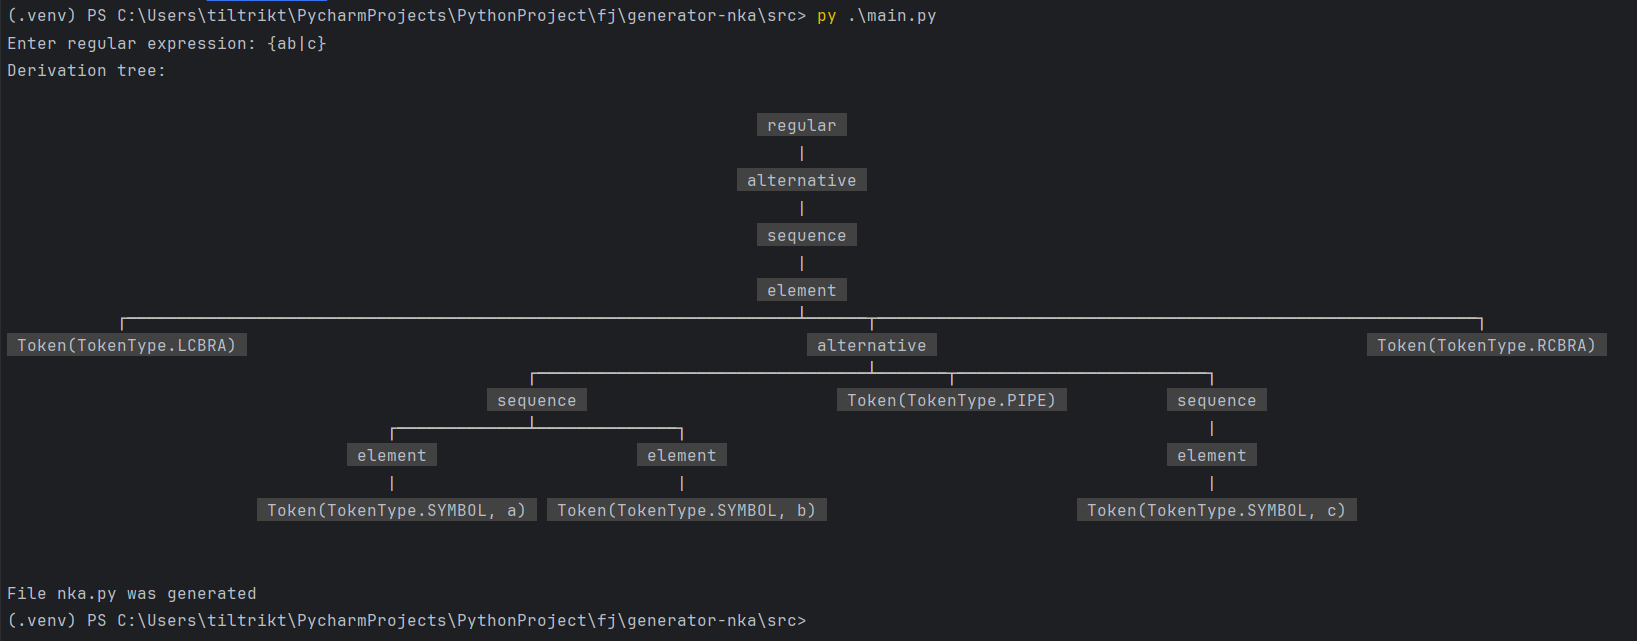
\includegraphics[width=1\textwidth]{figs/tree-example}
    \caption{Príklad vstupu}
    \label{fig:tree-example}
\end{figure}
Po spustení programu sa vygeneruje strom zobrazený na obrázku~\ref{fig:tree-example} a súbor \texttt{nka.py}.
Vygenerovaný súbor \texttt{nka.py} funguje nasledovne:
\lstset{basicstyle=\ttfamily}
\begin{lstlisting}
(.venv) PS ...\generator-nka\src> py .\nka.py
Enter a word:
Word '' is ACCEPTED!
Enter a word: ab
Word 'ab' is ACCEPTED!
Enter a word: c
Word 'c' is ACCEPTED!
Enter a word: ababcccabc
Word 'ababcccabc' is ACCEPTED!
Enter a word: acb
Word 'acb' is NOT ACCEPTED!
Enter a word: ab123
Word 'ab123' is NOT ACCEPTED!
Enter a word: quit
(.venv) PS ...\generator-nka\src>
\end{lstlisting}


\subsection{Problémy a ich riešenie}

Dlho mi trvalo, kým som pochopil, ako generovať tabuľku prechodov. Pokúsil som sa ju implementovať pomocou Thompsonovho konštrukčného algoritmu.
Týmto spôsobom som vytvoril menšie NKA, ktoré som následne spájal do jedného väčšieho automatu podľa definovaných pravidiel.
Po niekoľkých neúspešných pokusoch sa mi konečne podarilo implementovať generovanie tabuľky prechodov pre jednoduchý regulárny výraz \textit{ab}.
Preto som sa rozhodol pokračovať v tomto prístupe a rozširovať jeho funkčnosť pre zložitejšie regulárne výrazy.

\subsection{Hodnotenie zadania}

Úloha bola veľmi zaujímavá a pomohla mi lepšie pochopiť mnohé témy. Jediným problémom, s ktorým som sa stretol, bolo nájsť knižnicu na nakreslenie stromu. Ušetril by som veľa času, keby bolo niekoľko poskytnutých v samotnom zadaní.

\section{Vyhodnotenie a záver}

Podarilo sa mi implementovať všetko. Úloha sa testovala na niekoľkých rôznych vstupoch: správnych, nesprávnych a prázdnych. Nemusel som sa zaseknúť na žiadnom bode na dlhší čas.

\end{document}